\subsubsection{Hardware design}
This section covers the design of all of the mechanical hardware that was designed specifically for this project.\\

The first of the parts to be designed was the legs that would determine the scale of the robot. The legs were designed in three different segments as discussed in the theoretical and mathematical analysis. In order to simplify the mechanical design and distribute the weight of the robot more evenly, the servos are mounted inside the legs. Because the legs are lifted by the servos, these should be as close as possible to the hip in order to minimize the leverage on the servo lifting the leg.

\begin{figure}[H]
\centering
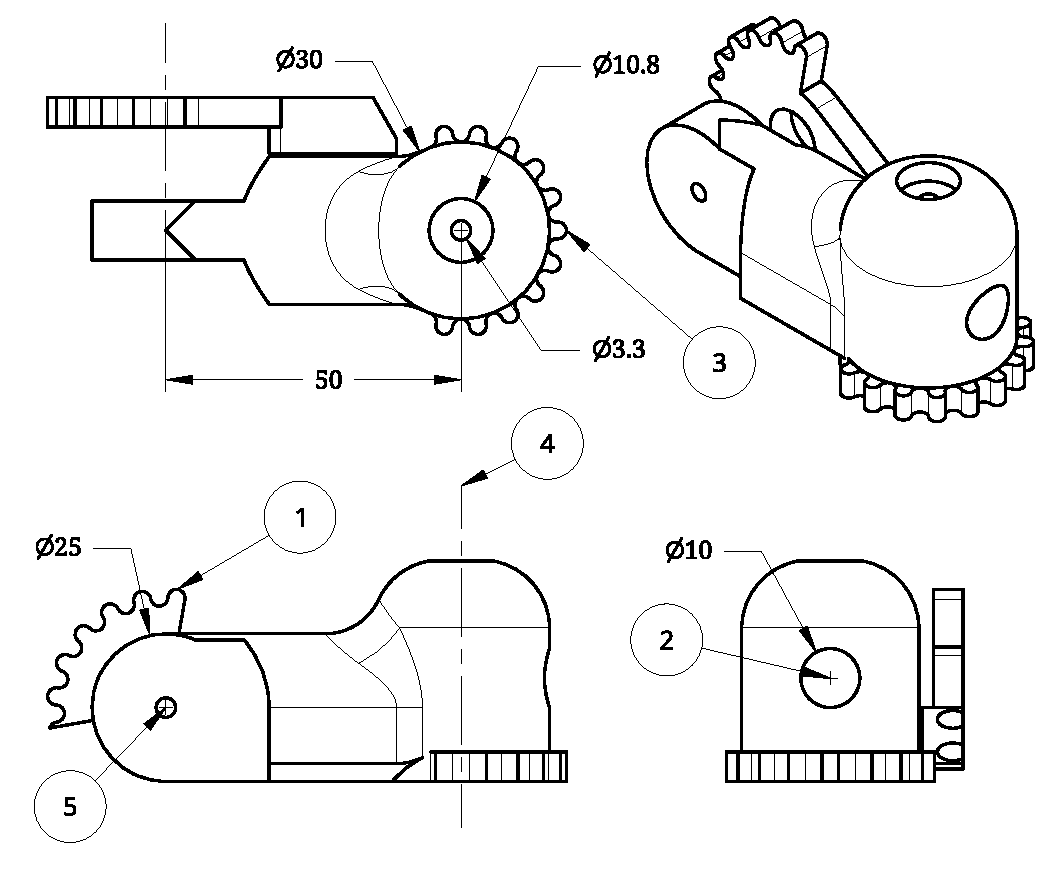
\includegraphics[scale = 0.8]{pics/DrawingA.pdf}
\caption{Illustration of how multiple servo motors are controlled using two timers.}
\label{fig:DrawingA}
\end{figure}

\begin{figure}[H]
\centering
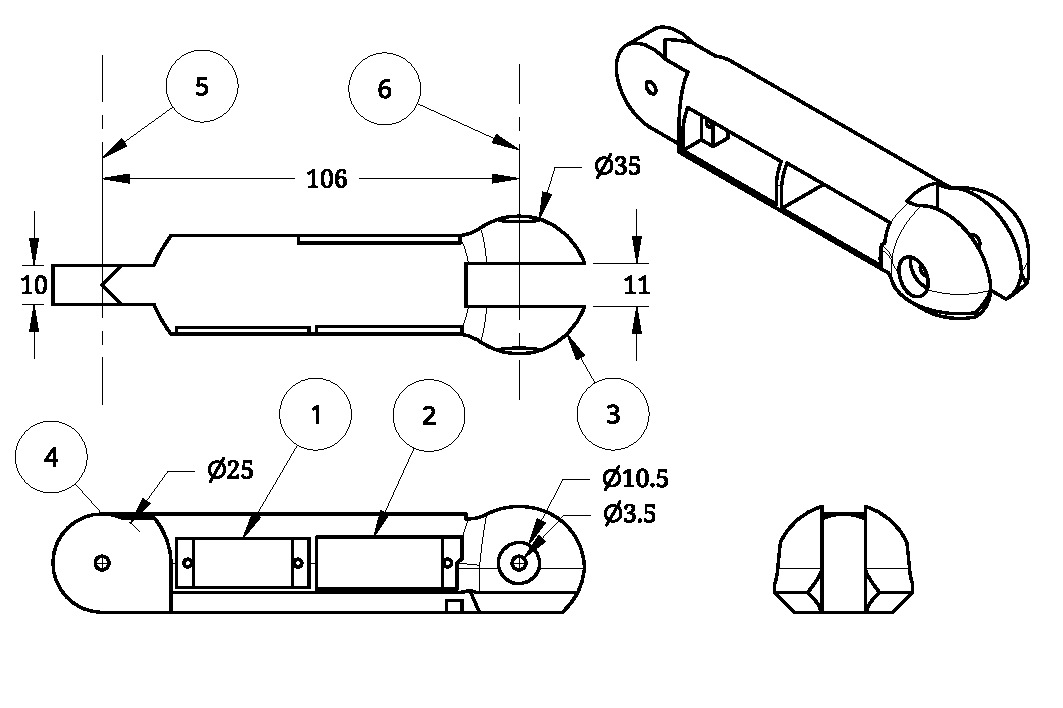
\includegraphics[scale = 0.8]{pics/DrawingB.pdf}
\caption{Illustration of how multiple servo motors are controlled using two timers.}
\label{fig:DrawingB}
\end{figure}

\begin{figure}[H]
\centering
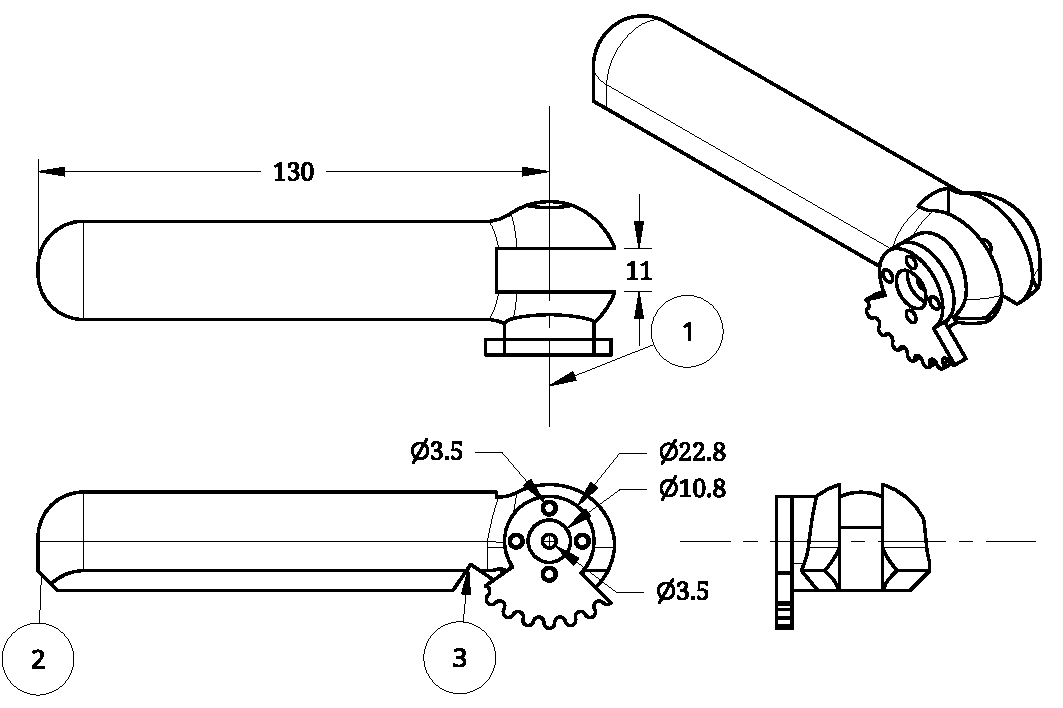
\includegraphics[scale = 0.8]{pics/DrawingC.pdf}
\caption{Illustration of how multiple servo motors are controlled using two timers.}
\label{fig:DrawingC}
\end{figure}

\begin{figure}[H]
\centering
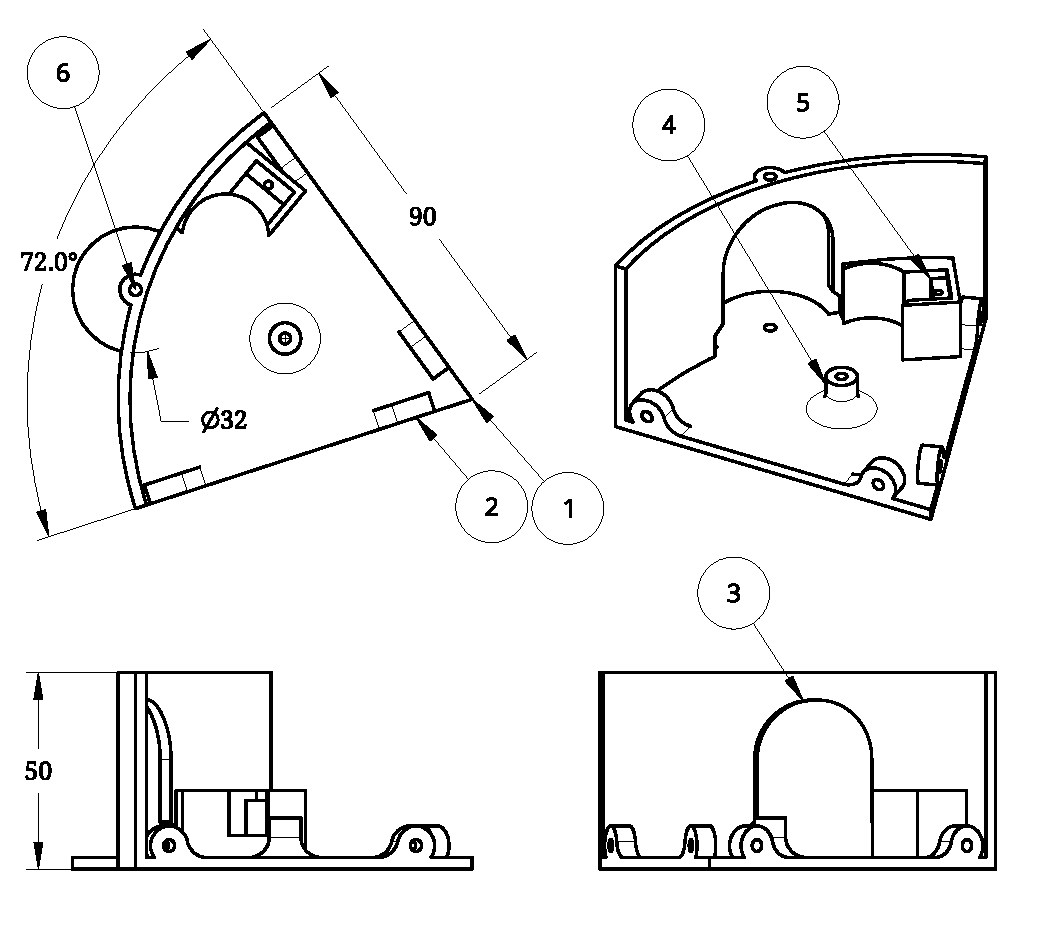
\includegraphics[scale = 0.8]{pics/DrawingBase.pdf}
\caption{Illustration of how multiple servo motors are controlled using two timers.}
\label{fig:DrawingBase}
\end{figure}

\subsubsection{Hardware implementation}

\begin{figure}[H]
\centering
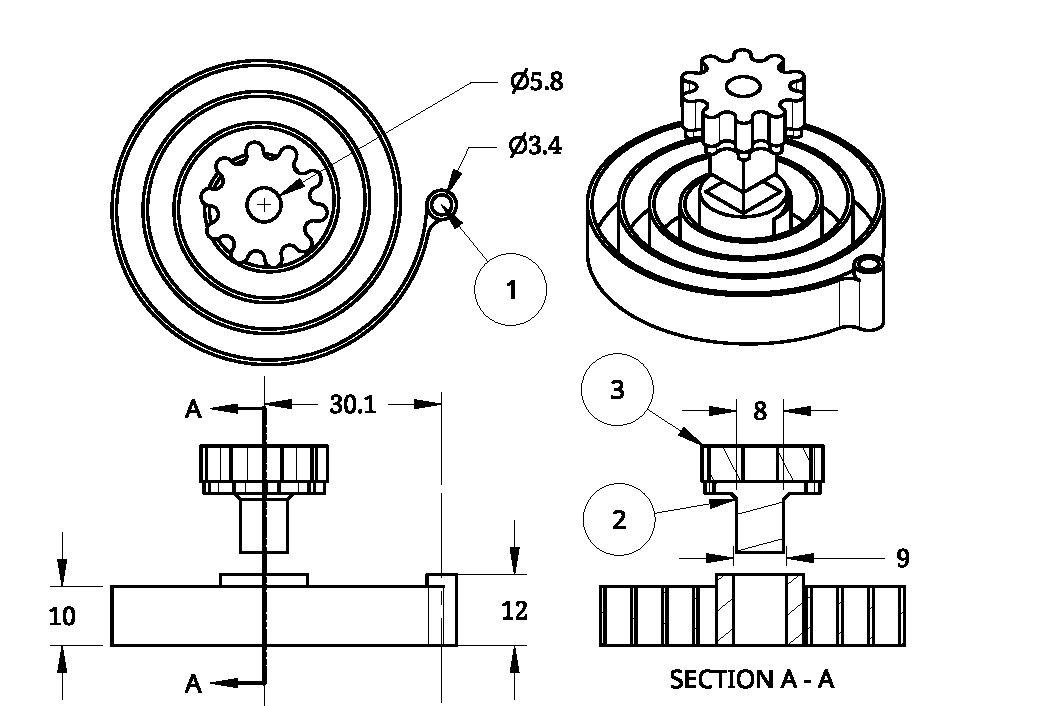
\includegraphics[scale = 0.8]{pics/DrawingSpring.pdf}
\caption{Illustration of how multiple servo motors are controlled using two timers.}
\label{fig:DrawingSpring}
\end{figure}